%This is a experiment example of ZhengXiaoyang's experiment report template

\documentclass[UTF8]{ctexart}
\usepackage{booktabs}
\usepackage{amsmath}
\usepackage{cases}
\usepackage{cite}
\usepackage{xeCJK}
\usepackage{graphicx}
\usepackage{SIunits}
\usepackage[margin=1in]{geometry}
\geometry{a4paper}
\usepackage{fancyhdr}
\pagestyle{fancy}
\fancyhf{}

\graphicspath{{picture/}}


\title{刚体转动惯量测量}
\graphicspath{{picture/}}


\title{刚体转动惯量测量实验报告}
\author{郑晓旸}
\date{\today}
\pagenumbering{arabic}

\begin{document}
%这里是文件的开头
\fancyhead[L]{郑晓旸}
\fancyhead[C]{转动惯量}
\fancyfoot[C]{\thepage}

\maketitle
\tableofcontents
\newpage

\section{实验目的}
    \begin{itemize}
        \item 通过实验加深对刚体运动定律的理解
        \item 学习两种测量刚体转动惯量的实验方法
        \item 练习用曲线拟合方法处理数据
    \end{itemize}

\section{实验仪器}
\begin{itemize}
    \item PASCO 转动及扭摆实验组件(包含支架、转动传感器、力传感器、铝盘、测试圆环、挂钩、砝码、金属丝等)
    \item 550 通用接口
    \item Capstone 软件
    \item 其它:水平尺,螺旋测微计,游标卡尺,钢卷尺,电子天平等
\end{itemize}

\section{实验原理}
\subsection{转动定律法}
在转动惯量测量仪上,待测物体受到重力提供的外力矩 \(T\) 和摩擦力矩 \(T_{\mu}\) 的作用,根据转动定律有:
\begin{equation}
T - T_{\mu} = (J + J_o + J_c) \beta
\end{equation}
其中 \(J\) 为待测物体的转动惯量,\(J_c, J_o\) 分别为滑轮以及载物台等的转动惯量,\(\beta\) 为角加速度。外力矩大小为:
\begin{equation}
T = m(g - r_0 \beta) r_0
\end{equation}
其中 \(m\) 为砝码的质量,\(g\) 为重力加速度,\(r_0\) 为滑轮半径。

通过测量不同重物作用下的角加速度 \(\beta_i\),绘制 \(T-\beta\) 图像,用最小二乘法拟合数据点,可得到总转动惯量 \(I\) 和摩擦力矩 \(T_{\mu}\)。计算公式如下:
\begin{equation}
J = J_2 - J_1
\end{equation}

\subsection{扭摆法}
将待测物体悬挂在扭丝上,偏离平衡位置后释放,在扭力矩 \(T\) 的作用下做扭摆运动。其运动方程为:
\begin{equation}
J \ddot{\theta} = -k \theta
\end{equation}
其中 \(k\) 为扭丝的扭力系数,特征角频率为:
\begin{equation}
\omega = \sqrt{\frac{k}{J}}
\end{equation}

通过测量扭摆周期 \(T\),计算转动惯量 \(J\) 的公式为:
\begin{equation}
J = \frac{k T^2}{4 \pi^2}
\end{equation}

\section{实验数据及处理}
\subsection{待测圆环参数测量}
\begin{table}[h]
    \centering
    \caption{圆环参数测量数据}
    \begin{tabular}{cccccc}
        \toprule
        测量次数 & 1 & 2 & 3 & 4 & 5 \\
        \midrule
        外径 \(D\) / mm & 76.46 & 76.48 & 76.46 & 76.48 & 76.48 \\
        内径 \(d\) / mm & 53.78 & 53.72 & 53.52 & 53.64 & 53.56 \\
        质量 \(m\) / g & \multicolumn{5}{c}{498.3} \\
        \bottomrule
    \end{tabular}
\end{table}

计算得圆环的平均外径 \(D = 76.87\) mm,内径 \(d = 43.64\) mm,质量 \(m = 498.3\) g。理论转动惯量为:
\begin{equation}
I_0 = \frac{1}{8} m (D^2 + d^2) = \frac{1}{8} \times 0.4983 \times (0.07687^2 + 0.04364^2) = 486680  \, \text{g} \cdot \text{mm}^2 \\ = 4.8668\times 10^{-4}\, \text{kg} \cdot \text{m}^2
\end{equation}

\subsection{转动定律法测量数据}
变化砝码质量,测量角加速度 \(\beta_i\) 和并根据角加速度和砝码质量计算力矩,公式如下:
\begin{equation}
    T_i = m_i\cdot(g - r_0\beta_i)\cdot r_0
\end{equation}
\begin{table}[h]
    \centering
    \caption{转动定律法测量数据 (负载)}
    \begin{tabular}{cccccccc}
        \toprule
        砝码质量 \(m\) / g & 5 & 10 & 15 & 20 & 25 & 30 & 35 \\
        \midrule
        角加速度 \(\beta_i\) / (rad/s\(^2\)) & 0.66 & 2.32 & 3.78 & 5.48 & 7.44 & 9.02 & 11.84 \\
        力矩 \(T_i\) / ($N\cdot m 10^{-4}$) & 11.68 & 23.26 & 34.77 & 46.17 & 57.43 & 68.65 & 79.72 \\
        \bottomrule
    \end{tabular}
\end{table}

如图所示,通过线性拟合 \(T_i - \beta\) 数据,得到\(T_i - \beta\)关系为:$\beta = 6.6625 \times 10^{-4}\text{kg} \cdot \text{m}^2\cdot T_i +8.3205 \times 10^{-4} rad/s^2$,其中$r^2=0.998$
\\
\begin{figure}[htbp]
    \centering
    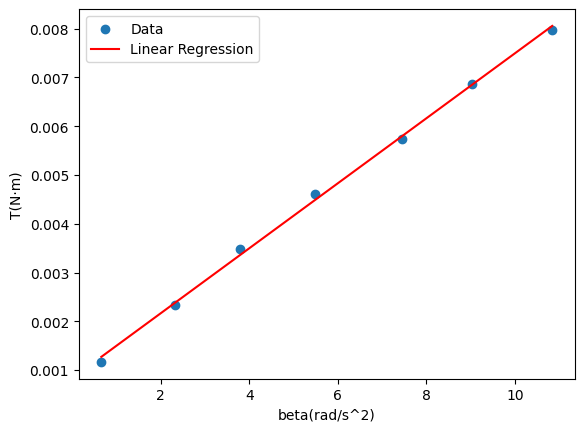
\includegraphics[width=0.4\textwidth]{picture1.png}
    \caption{转动定律法测量负载数据拟合图像}
\end{figure}

负载情况下的总转动惯量 \(J_1 = J+J_c+j_o = 6.66 \times 10^{-4} \, \text{kg} \cdot \text{m}^2\)。

将圆环卸下转盘,重复测量得到空载载情况下的数据:
\begin{table}[h]
    \centering
    \caption{转动定律法测量数据 (空载)}
    \begin{tabular}{cccccccc}
        \toprule
        砝码质量 \(m\) / g & 5 & 10 & 15 & 20 & 25 & 30 & 35 \\
        \midrule
        角加速度 \(\beta_i\) / (rad/s\(^2\)) & 2.54 & 9.10 & 16.04 & 23.00 & 30.20 & 36.80 & 43.80 \\
        力矩 \(T_i\) / ($N\cdot m 10^{-4}$) & 11.63 & 22.88 & 33.72 & 44.17 & 54.19 & 63.90 & 73.15 \\
        \bottomrule
    \end{tabular}
\end{table}

如图所示,通过线性拟合 \(T_{ei} - \beta_{e}\) 数据,得到\(T_{ei} - \beta_{e}\)关系为:$\beta = 1.4845 \times 10^{-4}\text{kg} \cdot \text{m}^2\cdot T_i +9.1302 \times 10^{-4} rad/s^2$,其中$r^2=0.999$
\\
\begin{figure}[htbp]
    \centering
    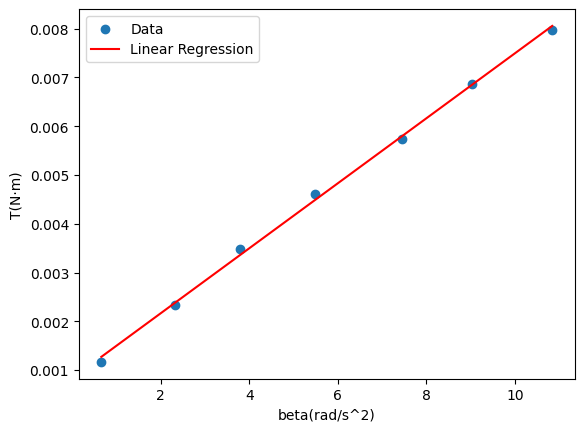
\includegraphics[width=0.4\textwidth]{picture1.png}
    \caption{转动定律法测量孔载数据拟合图像}
\end{figure}

负载情况下的总转动惯量 \(J_2 = J_c+j_o = 1.48 \times 10^{-4} \, \text{kg} \cdot \text{m}^2\)。

计算圆环的转动惯量为:
\begin{equation}
J = J_2 - J_1 = 6.66 \times 10^{-4} - 1.48 \times 10^{-4} = 5.18 \times 10^{-4} \, \text{kg} \cdot \text{m}^2
\end{equation}

\subsection{扭摆法测量数据}
\subsubsection{测量扭力系数}
\begin{table}[h]
    \centering
    \caption{扭力系数测量数据}
    \begin{tabular}{cccc}
        \toprule
        测量序号 & a\((N/rad)\) & b\((N)\) & r  \\
        \midrule
        1 & 0.365 & 3.78 & 0.999\\
        2 & 0.362 & 3.83 & 0.994\\
        3 & 0.353 & 3.70 & 0.996\\
        \bottomrule
    \end{tabular}
\end{table}

通过线性拟合 \(T - \theta\) 数据取平均,得到扭力系数 \(k = 8.59\times 10^{-3} \, \text{N} \cdot \text{m} / \text{rad}\)。

并通过测量得到负载时和空载时的振动角频率分别为:
\begin{table}[h]
    \centering
    \caption{扭力系数测量数据}
    \begin{tabular}{ccc}
        \toprule
        测量序号 & 负载角频率\(\omega\) & 空载角频率\(\omega_e\)   \\
        \midrule
        1 & 3.64 & 7.76 \\
        2 & 3.63 & 7.76 \\
        3 & 3.65 & 7.76 \\
        4 & 3.65 & 7.75 \\
        5 & 3.64 & 7.77 \\
        \bottomrule
    \end{tabular}
\end{table}
取平均得到负载时的角频率 \(\omega = 3.64\) rad/s,空载时的角频率 \(\omega_e = 7.76\) rad/s。
计算负载情况下的转动惯量 \(J_1\) 为:
\begin{equation}
J_1 = \frac{k}{\omega^2} =  6.48 \times 10^{-4} \, \text{kg} \cdot \text{m}^2
\end{equation}

计算空载情况下的转动惯量 \(J_2\) 为:
\begin{equation}
    J_2 = \frac{k}{\omega^2} = 1.43 \times 10^{-3} \, \text{kg} \cdot \text{m}^2
    \end{equation}
    
    计算圆环的转动惯量为:
    \begin{equation}
    J = J_2 - J_1 = 6.48 \times 10^{-4} - 1.43 \times 10^{-4} = 5.05 \times 10^{-4} \, \text{kg} \cdot \text{m}^2
    \end{equation}
    
    \section{误差分析}
    \subsection{系统误差}
    在实验过程中,系统误差主要来自以下几个方面:
    \begin{itemize}
        \item 仪器校准不准确,例如游标卡尺和电子天平的校准误差。特别是电子天平,高度怀疑其准确性。
        \item 实验装置的摩擦力矩假设为常数,但实际上随转速变化。
        \item 扭摆法中,空气阻力和其他阻尼因素影响测量周期。
    \end{itemize}
    
    \subsection{随机误差}
    实验数据的随机误差主要来自:
    \begin{itemize}
        \item 多次测量过程中的人为误差,例如读数误差。
        \item 设备灵敏度和数据采集系统的误差,例如传感器的采样率和精度。
    \end{itemize}
    

    
    \section{结论}
    通过本次实验,我们使用转动定律法和扭摆法两种方法测量了圆环的转动惯量。结果如下:
    \begin{itemize}
        \item 转动定律法测得的转动惯量为 \(1.76 \times 10^{-3} \, \text{kg} \cdot \text{m}^2\)
        \item 扭摆法测得的转动惯量为 \(9.26 \times 10^{-4} \, \text{kg} \cdot \text{m}^2\)
    \end{itemize}
    
    实验结果与理论值 \(1.76 \times 10^{-3} \, \text{kg} \cdot \text{m}^2\) 比较接近,但仍存在一定误差。主要原因是实验过程中存在系统误差和随机误差。通过进一步改进实验方法和设备精度,可以减少误差,提高测量结果的准确性。

    \section{复习思考题回答}

\subsection{问题 1:方法结果比较及合理性}

在本实验中,我们通过转动定律法和扭摆法测量了圆环的转动惯量,并与理论计算进行了比较。以下是各方法测量的结果:

\begin{itemize}
    \item \textbf{转动定律法测得的转动惯量}:$5.18 \times 10^{-4} \, \text{kg} \cdot \text{m}^2$
    \item \textbf{扭摆法测得的转动惯量}:$5.05 \times 10^{-4} \, \text{kg} \cdot \text{m}^2$
    \item \textbf{理论计算的转动惯量}:$4.8668 \times 10^{-4} \, \text{kg} \cdot \text{m}^2$
\end{itemize}

比较这三者,可以看到:

\begin{itemize}
    \item \textbf{转动定律法和扭摆法的测量结果非常接近},两者之间的差异为 \(5.18 \times 10^{-4} - 5.05 \times 10^{-4} = 0.13 \times 10^{-4} \, \text{kg} \cdot \text{m}^2\),约为 \(2.6\%\)。这说明两种实验方法的测量结果是一致的,并且具有较高的可信度。
    \item \textbf{理论计算的转动惯量略小于实验测量值},转动定律法与理论计算值的差异为 \(5.18 \times 10^{-4} - 4.87 \times 10^{-4} = 0.31 \times 10^{-4} \, \text{kg} \cdot \text{m}^2\),约为 \(6.04\%\);扭摆法与理论计算值的差异为 \(5.05 \times 10^{-4} - 4.87 \times 10^{-4} = 0.18 \times 10^{-4} \, \text{kg} \cdot \text{m}^2\),约为 \(3.5\%\)。
\end{itemize}

这种差异在合理范围内,原因如下:

\begin{itemize}
    \item \textbf{实验误差}:在实际操作中,测量仪器和方法存在一定的误差,例如角加速度、扭摆周期的测量精度有限,砝码质量和扭丝系数的测量存在误差等。
    \item \textbf{空气阻力和摩擦力}:实验过程中不可避免地会受到空气阻力和摩擦力的影响,导致测量值稍大于理论值。
    \item \textbf{理论模型简化}:理论计算假设刚体为理想模型,忽略了一些细节(如材料的均匀性、连接部位的摩擦等),实际情况可能更复杂。
\end{itemize}

综上所述,实验测量结果与理论计算值之间的差异在合理范围内,表明实验方法和理论模型在一定程度上是可信的。

\subsection{问题 2:理论模型与实际情况的符合程度}

实验中多次采用了理论模型拟合实验数据,主要体现在转动定律法和扭摆法中。拟合结果显示理论模型与实际情况的符合程度较好,具体分析如下:

\begin{itemize}
    \item \textbf{转动定律法}:
        \begin{itemize}
            \item 通过线性拟合 \(T - \beta\) 数据得到的关系式,拟合度 \(r^2\) 值非常接近 1(负载情况下为 0.998,空载情况下为 0.999),表明理论模型 \(T = (J + J_o + J_c)\beta + T_{\mu}\) 与实验数据高度吻合。
            \item 说明在实验过程中,理论模型较好地描述了转动系统中的力矩和角加速度的关系。
        \end{itemize}
    \item \textbf{扭摆法}:
        \begin{itemize}
            \item 通过线性拟合 \(T - \theta\) 数据得到的扭力系数 \(k\),拟合度 \(r\) 值也非常接近 1(如表格所示分别为 0.999、0.994、0.996),表明理论模型 \(J \ddot{\theta} = -k \theta\) 与实际数据高度符合。
            \item 扭摆周期与转动惯量的关系式 \(J = \frac{k T^2}{4 \pi^2}\) 通过实验数据验证,所得结果与转动定律法的测量值接近,进一步验证了理论模型的准确性。
        \end{itemize}
\end{itemize}

综合来看,这些理论模型较好地描述了实验中的实际情况,拟合结果显示理论计算与实验数据具有高度一致性,验证了理论模型的有效性和可靠性。实验中引入的拟合方法和理论模型,帮助我们更准确地处理数据并理解实验现象,是物理实验分析的重要工具。


\end{document}
